\chapter{Artworks}

%%%
%%%
%%%
\section{Collage, Assemblage and the Found Object}
In this chapter root of using objects in the artworks is examined. Using objects on artworks beyond their intended purpose. Developing artworks not only painting but also using paper and other stuff by pasting them together.

%%
%%
\subsection{Collage}
Collage originates from the French \textit{coller} is an artistic technique of applying manufactured, printed, or “found” materials, such as bits of newspaper, fabric, wallpaper, etc., to a panel or canvas, frequently in combination with painting. In about 1912–13 Pablo Picasso and Georges Braque extended this technique, combining fragments of paper, wood, linoleum, and newspapers with oil paint on canvas to form compositions. Pasting paper is not a new technique but using this it in the art making is a revolutionary movement in the  language of art \cite{waldman1992collage}.

\cite{greenberg1984collage}

%%
%%
\subsection{Assemblage}
Assemblage work produced by the incorporation of everyday objects into a composition. It is similar to collage, but main difference is that assemblage is three dimensional rather collage is two-dimensional. Diverse range of things can be used production of work. In 1961, the exhibition "The Art of Assemblage" was featured at the New York Museum of Modern Art. William C Seitz, the curator of the exhibition, described assemblages as being made up of preformed natural or manufactured materials, objects, or fragments not intended as art materials \cite{seitz1961art}.

%%
%%
\subsection{Found Object (Ready-mades)}
Found object originates from the French \textit{objet trouvé}, describing art created from undisguised, but often modified, objects or products that are not normally considered art, often because they already have a non-art function. Pablo Picasso first publicly utilized the idea when he pasted a printed image of chair caning onto his painting titled Still Life with Chair Caning (1912). Marcel Duchamp is thought to have perfected the concept several years later when he made a series of ready-mades, consisting of completely unaltered everyday objects selected by Duchamp and designated as art. The most famous example is Fountain (1917), a standard urinal purchased from a hardware store and displayed on a pedestal, resting on its side.

%%
%%
\subsection{Bricolage}
Something constructed using whatever was available at the time.

Claude Levi-Strauss notes: the bricoleur works not from the principle of making things only if natural resources are available but makes things according to those things at hand, making do with what is available. It is an expression that, like the natural cycles of the Earth, attempts to make something new from something old. \cite{levi1966savage}

\cite{strasser1999waste}

%%
%%
\subsection{Folk Art}
In contrast to fine art, folk art is primarily utilitarian(practical and functional, not just for show) and decorative rather than purely aesthetic. The nature of folk art is specific to its particular culture.

%%
%%
\subsection{Art and activism}


%%
%% TODO change here
\subsection{History of Consumption and Waste}
"The use of trash as a fine art medium dates back at least to the work of early-20th-century artists such as Fortunato Depero and Kurt Schwitters. Use of found materials, including garbage, has been associated with assemblage art since the 1950s and has been practiced by other well-known artists, including graphic artist Christian Boltanski, sculptor Louise Bourgeois, and photographer Andres Serrano. Art made from garbage has since become much more common in fine arts venues such as museums, galleries, and high-profile installations, including H. A. Schuldt’s famous “Trash People,” which has traveled around the world since 1996." \cite{tauxe2012encyclopedia}

%%
%% TODO change here
\subsection{Discussion}
Are artworks made from trash just examples of collage and assemblage or more than from them? What about the experience and interaction with other people? Turning art making process to a life practice (or part of life) can be explained in the context of collage (which is mainly related with how a 2d canvas created). But all of them work in fragments, combine many objects together. 

Garbage is often viewed as a form of society’s excess---as the unwanted things that are thrown out without regard. 

In the world of computer science, the term garbage also refers to situations of loss in which data or objects in memory go unused in computer operations.

%%%
%%%
%%%
\section{Artworks}
Artist and artworks related with trash and their analysis. Stages of their works and methods.

% FROM ReVista
Trash is dirty. Trash is smelly. Trash can provide the raw materials for exquisite art---from sculpture to film and beyond.

% FROM Paola Ibarra ReVista
Whether in sculpture, photography or other media, art frequently deals, directly or by allusion, with daily challenges of life in Latin America and elsewhere. Is there a limit to recycling and representation? Or is there a point at which waste cannot become art (or anything else)?

\begin{itemize}
% FROM Maite Zubiaurre, ReVista Garbage
\item Filomena Cruz creates photographic series “Road Kill” painstakingly captures tiny “trash corpses” on the pavement. It is that particular type of trash meet in the public places. trash left behind, trash on the sidewalk, squished, squashed, and weathered. Filomena Cruz sees trash that we don’t want to see. A
piece of chewing gum with an “engraved” leaf; a flattened-out tube; a corroding paper napkin with a still intact heart; or a frog-green Crayola melting in the heat, all speak the language of “worthlessness” suddenly becoming meaningful (and moving).For one thing, trash corpses faithfully record city life. 
  \begin{figure}[ht]
      \centering
      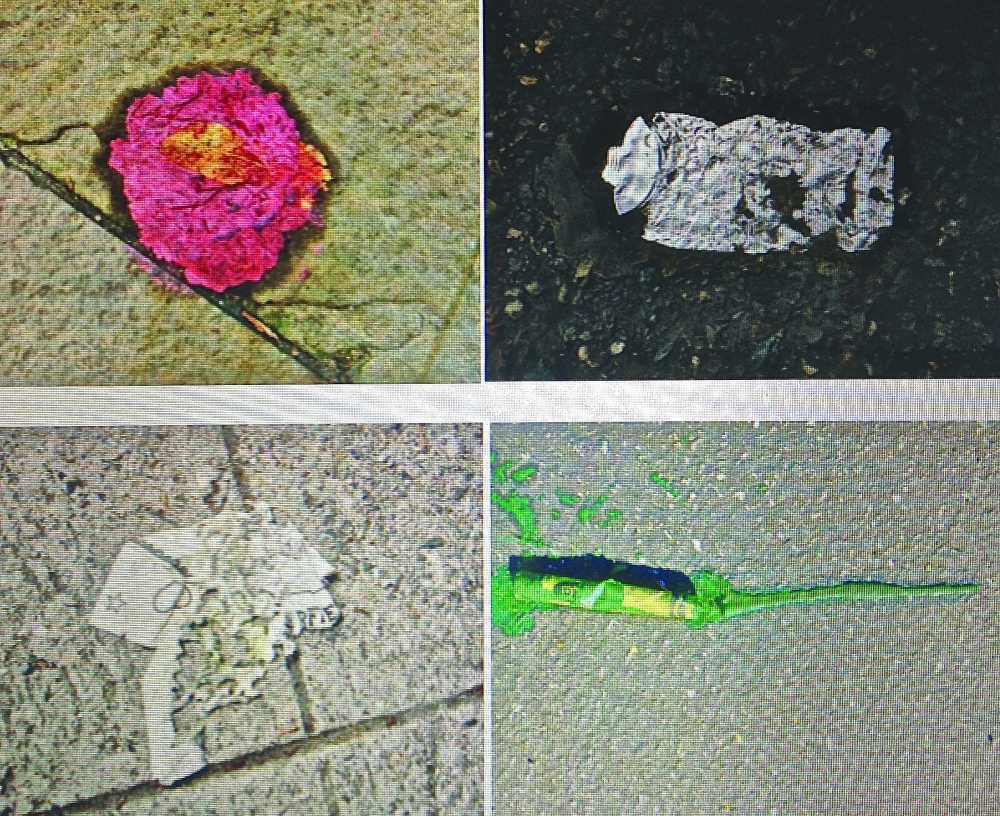
\includegraphics[width=0.8\textwidth]{graphics/FilomenaCruz_RoadKill_ReVista.jpg}
      \caption{Road Kill by Filomena Cruz}
      \label{fig:FilomenaCruz_RoadKill_ReVista}
  \end{figure}

\item Vic Muniz creates monumental trash art in Jardim Gramacho with the help of \textit{catadores} (Waste Land, 2010)

% https://www.youtube.com/watch?v=sJxxdQox7n0
\item Favio Chávez and Nicolás Gómez decide to build musical instruments out of garbage and get 35 children from Cateura, Paraguay’s biggest trash dump, to travel the world with their “Recycled Orchestra,” or “Landfill Harmonic”.

% http://www.eloisacartonera.com.ar/ENGversion.html
\item “Eloísa Cartonera,” a work cooperative in Buenos Aires, proudly produces handmade books with cardboard covers: \quotes{We purchase [\ldots] cardboard from the
urban pickers (\textit{cartoneros}) who pick it from the streets. Our books are on Latin American literature, the most beautiful we had a chance to read in our lives.} \quotes{Some of them are preserved as art books at university libraries, while others circulate as literary pieces expected to disintegrate in time---something anticipated of the material they are made from.} [from PAOLA IBARRA, ReVista]
  \begin{figure}[ht]
      \centering
      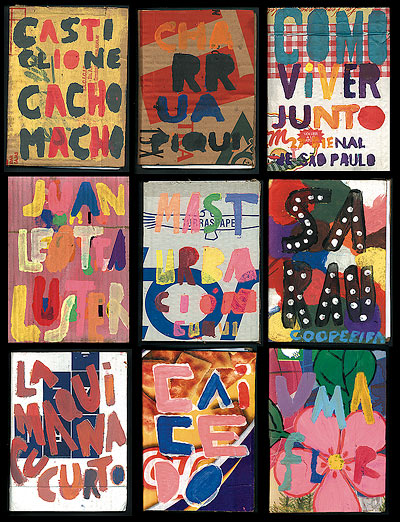
\includegraphics[width=0.8\textwidth]{graphics/EloisaCartonera_Books.jpg}
      \caption{Books covered by Eloisa Cartonera}
      \label{fig:EloisaCartonera_Books}
  \end{figure}

% FROM Paola Ibarra, ReVista
%\item Forever; Blue Yonder by artist Kyle Huffman
%\item Too Too---Much Much by Thomas Hirschhorn
%\item Autoconstrucción by Abraham Cruzvillegas
%\item Pictures of Garbage by Vik Muniz

% FROM Daniel Lind-Ramos BY LOWELL FIET, ReVista
%\item Daniel Lind-Ramos

% FROM A Present from the Sea BY SONIA CABANILLAS, ReVista
% https://www.youtube.com/watch?v=v6IoEF_Tsrw
\item Nick Quijano has some rules to create assemblages. \quotes{There are certain self-imposed rules to this creative process: first, the assemblages or artefactos must all come from material washed ashore on this beach; second, it must be plastic and industrial refuse, result of the processing of fossil fuel; third, it must be polished by a long stay in deep waters, sometimes even encrusted with corals, shells or pebbles, or simply scraped by the ocean floor. As a sign of respect and sacralization, these pieces will be incorporated without any adjustment: no cutting or bending, seen as a mutilation of the object. Its identity cannot be veiled or masked but always must be recognizable amidst the other components; e.g, a comb must remain a comb even as one may see it as a mustache.} The sea returns this refuse; it is not biodegradable.

% FROM Burning Messages BY MICHAEL WELLEN, ReVista
%\item Antonio Berni

% FROM Haiti in the Time of Trash BY LINDA KHACHADURIAN, ReVista
\item Haiti case. When I ask him why he chooses to work in the medium of trash, he replies, \quotes{It gives respect to my city to use the garbage. It shows that everything can be used, and nothing was lost.} (TODO motivation: \quotes{I get more inspiration working with recycled materials because those pieces are unique and can’t be duplicated}) Eugène says that he’s partial to metal, which has become more and more difficult to find because of the clean-up initiative by the city. When I ask him if part of him wishes there were no such effort underway, he answers: \quotes{No. When you have clean streets you have good health, and that is the most important thing.} (This is very strange. It shows that working with trash and being clean healthy is not a contradiction. Both of them exist together.) \quotes{Other people come to Haiti and see junkyards, but we see magical playgrounds,} Jean explains as he watches them.

% FROM Thinking on Film and Trash BY ERNESTO LIVON-GROSMAN, ReVista
% By the 1950s a film like Tire Dié (Fernando Birri, Argentina, 1956) already portrays the collecting, classifying and recycling of trash not only as a source of informal income but as a commercial activity linked to the formal economy. In these films, trash is not the end of a process of consumption but the beginning of a cycle of production. These movies share the idea that trash could be a departure point to think about the modern condition as defined by consumption, class disparities, contamination and urban development. The poet Charles Baudelaire is one of the first to make the connection between the rag picker and the modern city. Walter Benjamin picks it up and from then on the fragmentary condition of trash will remain associated with contemporary art and ultimately with the Modern condition: the industrial refuse could be redeemed by art. It is in this sense that filmmaking becomes allegorical and mimics the process of recycling when it reappropiates archival materials and found footage to create new narratives from scraps, fragments, of films that were not in any way connected to these new narratives.

\item Joseph Cornell

\item \textbf{American Beauty.} The film American Beauty , which features a long, poetic clip of a plastic bag swirling on an eddy of air, snagged five Academy Awards, yet I for one still find it hard to think of plastic bags as things of beauty. 

\item \textbf{Aaron Kramer.} His motto: "Trash is the failure of imagination." \cite{meyer2007turning}

\end{itemize}

Childs can enjoy with trash. I remember from my childhood, we collect crown cap and play with them. Some caps are found less and they worth more. We are looking everywhere for them. To make them flat we put them on the railways. After train passed we get perfect plat cap. At that time it is not trash for us. It has a value and part of our games and enjoy. To have fun a bunch of trash can be enough for us.

In the case of recycling, a dead objects, or an object that reached end of life will begin a new cycle of life. By the artist or other parts are give them a new life. They can reborn as a different things. Do people collect them aware of it? Discarded items unites together with the hands of a artist. 

Trash is global topic men. When you talk about trash, everyone have ideas about it. 

Think a city that has trash monument in the every corner. created from their trash. merged with the city life and gaining unique cityscapes and aesthetics. or think that a museum a trash museum. Exhibits works of art embracing the trash in all aspects. Maybe done by the artist or the visitors from all around world. A place for garbage other than a landfill. Waiting their creator to meet again. What a great idea isn't it? Meeting their creators again. But this time their creator can recognize their trash. They transformed to totally new thing. Reborn. Transformed (Kafka, Gregor Samsa).

%%
%%
\subsection{Artist statements}

%%
%%
\subsection{What might be the meaning of using trash as a medium in the artworks? Questioning trash as a medium for artist}
\begin{itemize}
\item Some works try to raise awareness the problems that are the result of trash. (It treats environment and nature.)
\item Some of them reflect people's lifestyle especially throw away culture. As a mirror of current lifestyle.
\item Try to find a new value and meaning from the discarded material that are useless anymore. To explore a new approach, new way. Subvert people's ideas about trash and their attitudes by turning materials to the something meaningful (or valuable). Trash to treasure.
\item Using discarded item to represent other discarded things by the ruling ideology or approach. For example, trash can be used to represent refugees. The things that we are trying to discard does not mean that they have no value, instead it means that we have no ability to reveal its potential. In other words, refugees have potential but we see them as players that will change our current system. Therefore, it can be said that willing to transform trash to treasure is to require change of current lifestyle. Rejecting discarding something especially thing that you get value from it is a process and spread through to the ones life.
\item One way is not to produce trash. (Zero trash philosophy.) The other one is to transform trash into something else.
\item What type of experience is that collecting and working on objects that are generally discarded? Experiencing out of common practice, being open to new explorations.
\item Instead of a world that produce trash, how could it be a world created from trash?
\item Combining industrial goods with objects transformed from trash is another way to find a place to trash in the community. It also signifies that trash still has a good quality to used with new materials. Creating composite products from new and reused items. Using the valuable thing with the invaluable thing. It becomes more valuable or less valuable. Depends on the perception.
\item Aesthetics of trash. Revealing aesthetics value of discarded stuff. (Unique visual value. Trash portraits, sculptures etc.)
\end{itemize}

\subsection{Artistic tactics}

